\section{Result}
In this experiment, two constraints are imposed on the composite laminates which are the safety
factor $CT_1$ for Tsai-Wu, and safety factor $CT_2$ for maximum stress. Both of them value is 1. The
constraint values of an individual are $CV_1$ and $CV_2$. So the mutation vector here is a two
dimensional vector $[1 - CV_1, 1 - CV_2 ]$, and the coefficient of length mutation $C_l$ and angle mutation
$C_a$, respectively, chosen here is 20 and 10. 

\begin{figure}[!t]
	\centering
		\begin{subfigure}[b]{0.8\linewidth}
			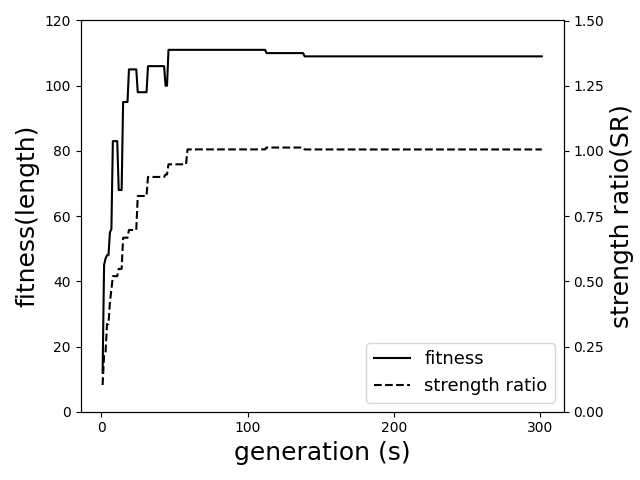
\includegraphics[width=\linewidth]{2020-11-10-pre-image/two_distinct_angle_fitness_and_sr.png}
		\end{subfigure}

		\begin{subfigure}[b]{0.8\linewidth}
			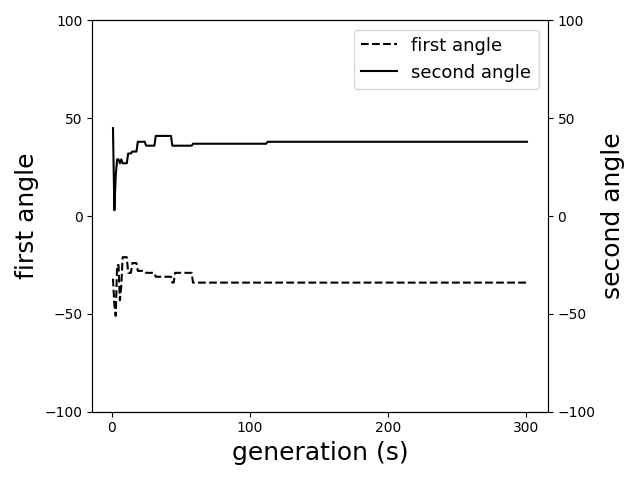
\includegraphics[width=\linewidth]{2020-11-10-pre-image/two_distinct_angle_angle_change.png}
		\end{subfigure}

		\begin{subfigure}[b]{0.8\linewidth}
			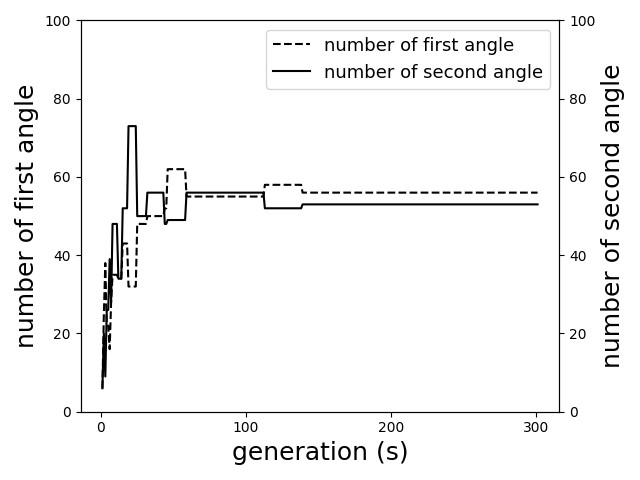
\includegraphics[width=\linewidth]{2020-11-10-pre-image/two_distinct_angler_number_change.png}
		\end{subfigure}
	\caption{Two distinct angles}
	\label{fig:two_angles}
\end{figure}



Figure \ref{fig:two_angles} (a) shows how the optimal individual's fitness and strength
ratio vary during the GA process. The method to chose optimal individual considering two following
situations, if no individual in the current population meets constraint, the one with biggest
fitness is selected as the optimal individual; if there are one or multiple individuals fullfils
requirement, the one with smallest fitness is chosen.  Figure \ref{fig:two_angles} (b) shows how the two distinct fiber
orientation changes at the same time, and Figure  \ref{fig:two_angles} (c) how the number of each angles change.

	At the beginning of this GA process, the fitness curves increased very quickly, becasue of
individual's strength ratio $CT_0$ is very small, so the difference between the individual's fitness and
the imposed constraint threshold is a big positive number, so the range of mutaion length is from 0
to $C_l(CT_0 - CV_0)$. The length of individual increases by n, which is random number between 0 and 
$C_l(CT_0 - CV_0)$. As can be seen from Figure \ref{fig:two_angles} (a), both of optimal
individual's fitness and strength ratio increases very quickly.  The range of mutaion angle is from
0 to $C_a(CT_0 - CV_0)$, and the number of every angle also change violently. During this stage,
increasing individual's length playing a major role in increasing individual's fitness.

After a couple of generations, the optimal individual's fitness get bigger, and the difference
between individual's fitness and constraint threshold get smaller. The range of mutaion length $[0,
C_l(CT_0 - CV_0)]$ turn smaller. At this stage, simply increase the individual's length doesn't make
much difference in improve individual's fitnees, and a better composite laminates lay-up can
dramaticly change the optimal individual's fitness. That's why the fitness curve oscillated
violently in this stage.  At the same time, the strength ratio curve kept growing smoothly. But the
growing speed got more smaller.

When GA comes to its last phase, GA found individuals that meet the constraint. Now the optimal
individual's fitness is greater than the safety factor. The range of mutation length is from 
$C_l(CT_0 - CV_0)$ to 0. It means individuals need to decrease it's length and improve its internal
structure to meet the constraint. That's why the fitness of optimal individual kept decreaing,
however, the strength ratio curve still is greater then safety factor.

\begin{figure}[!t]
	\centering
		\begin{subfigure}[b]{0.8\linewidth}
			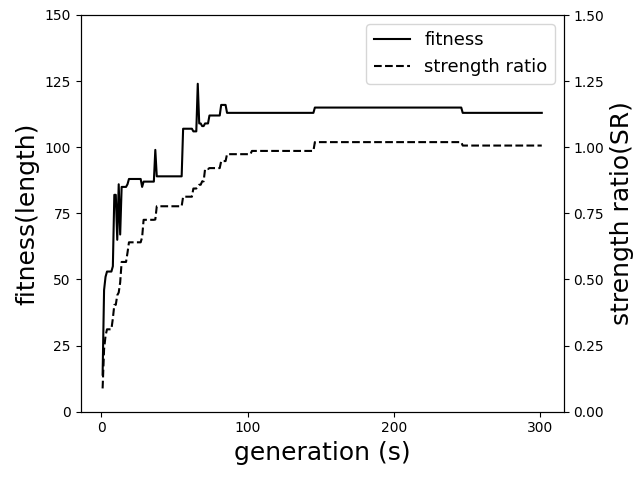
\includegraphics[width=\linewidth]{2020-11-10-pre-image/Three_distinct_angles_fitness_and_sr.png}
		\end{subfigure}

		\begin{subfigure}[b]{0.8\linewidth}
			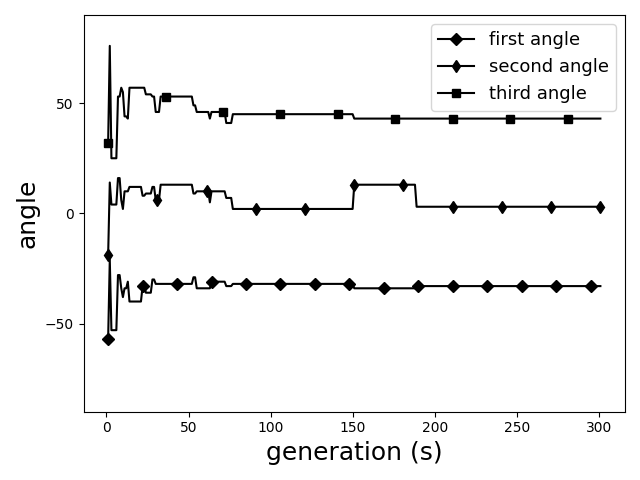
\includegraphics[width=\linewidth]{2020-11-10-pre-image/three_distinct_angles_angle_change.png}
		\end{subfigure}

		\begin{subfigure}[b]{0.8\linewidth}
			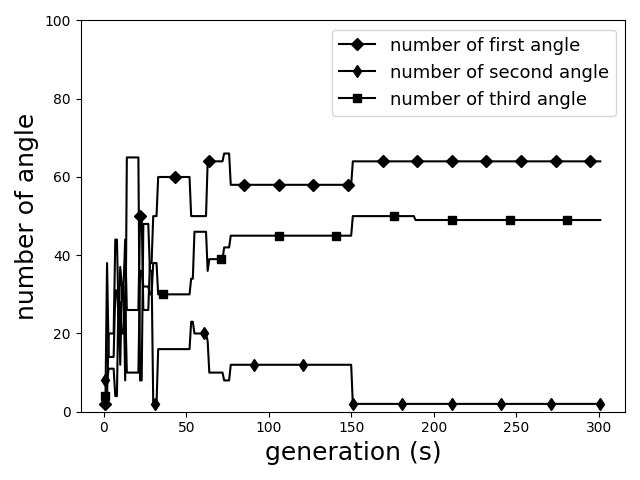
\includegraphics[width=\linewidth]{2020-11-10-pre-image/three_distinct_angle_number_of_angle.png}
		\end{subfigure}
	\caption{Three distinct angles}
	\label{fig:three_angles}
\end{figure}



\begin{table*}
%% increase table row spacing, adjust to taste
%\renewcommand{\arraystretch}{1.3}
% if using array.sty, it might be a good idea to tweak the value of
% \extrarowheight as needed to properly center the text within the cells
\caption{An Example of a Table}
\label{T300/5308 material properties}
\centering
%% Some packages, such as MDW tools, offer better commands for making tables
%% than the plain LaTeX2e tabular which is used here.
\begin{tabular}{cccc}
	\toprule
	Property								   & Symbol				  & Unit  &  Graphite/Epoxy     \\
	\midrule
	Longitudinal elastic modulus			   & $E_1$				  & GPa   &  181                 \\
	Traverse elastic modulus				   & $E_2$				  & GPa   &  10.3                \\
	Major Poisson's ratio					   & $v_{12}$			  &       &  0.28                \\
	Shear modulus							   & $G_{12}$			  & GPa   &  7.17                \\
	Ultimate longitudinal tensile strength     & $(\sigma_1^T)_{ult}$ & MP    &  1500                 \\
	Ultimate longitudinal compressive strength & $(\sigma_1^C)_{ult}$ & MP    &  1500                 \\
	Ultimate transverse tensile strength       & $(\sigma_2^T)_{ult}$ & MPa   &  40                   \\
	Ultimate transverse compressive strength   & $(\sigma_2^C)_{ult}$ & MPa   &  246                   \\
	Ultimate in-plane shear strength           & $(\tau_{12})_{ult}$  & MPa   &  68                    \\
	Density                                    & $\rho$               & $g/cm^3$ &  1.590                    \\
	\bottomrule
\end{tabular}
\end{table*}


% Note that IEEE does not put floats in the very first column - or typically
% anywhere on the first page for that matter. Also, in-text middle ("here")
% positioning is not used. Most IEEE journals/conferences use top floats
% exclusively. Note that, LaTeX2e, unlike IEEE journals/conferences, places
% footnotes above bottom floats. This can be corrected via the \fnbelowfloat
% command of the stfloats package.


\begin{table*}
%% increase table row spacing, adjust to taste
%\renewcommand{\arraystretch}{1.3}
% if using array.sty, it might be a good idea to tweak the value of
% \extrarowheight as needed to properly center the text within the cells
\caption{The optimum lay-ups using two distinct fiber angles under various biaxial loading cases}
\label{tab:two_distinct_angle}
\centering
%% Some packages, such as MDW tools, offer better commands for making tables
%% than the plain LaTeX2e tabular which is used here.
\begin{tabular}{ccccc}
	\toprule
	Loading	$N_{x}/N_{y}/N_{xy}$ (MPa m)	       & Optimum lay-up sequences                                   & laminate thickness &  Safety factor  & MS\\
	\midrule
	10/5/0                                         &  $[33_{29}/\text{-}39_{25}/\bar{\text{-}39}]_s$            &     109               &  1.0074      &  1.0246  \\
	20/5/0                                         &  $[33_{22}/\text{-}31_{24}]_s$                             &     92               &  1.0055       &  1.2065    \\
	40/5/0                                         &  $[29_{18}/\text{-}21_{23}/\bar{\text{-}21}]_s$            &     83               &  1.0034       &  1.7350   \\
	80/5/0                                         &  $[\text{-}20_{27}/21_{25}/\bar{25}]_s$                    &     105               &  1.0029      &  1.2063    \\
	120/5/0                                         &  $[\text{-}18_{34}/17_{36}]_s$                            &     140               &  1.0000      &  1.0898    \\
	\bottomrule
\end{tabular}
\end{table*}

\begin{table*}
%% increase table row spacing, adjust to taste
%\renewcommand{\arraystretch}{1.3}
% if using array.sty, it might be a good idea to tweak the value of
% \extrarowheight as needed to properly center the text within the cells
\caption{The optimum lay-ups using three distinct fiber angles under various biaxial loading cases}
\label{T300/5308 material properties}
\centering
%% Some packages, such as MDW tools, offer better commands for making tables
%% than the plain LaTeX2e tabular which is used here.
\begin{tabular}{cccc}
	\toprule
	Loading	$N_{x}/N_{y}/N_{xy}$ (MPa m)	       & Optimum lay-up sequences                                   & laminate thickness &  Safety factor \\
	\midrule
	10/5/0                                         &  $[37_{27}/\text{-}38_{27}/\text{-}5]_s$                   &     110               &  1.0023 \\
	20/5/0                                         &  $[34_{24}/\text{-}32_{14}/\text{-}28_{11}]_s$             &     98               &  1.0237 \\
	40/5/0                                         &  $[21_{28}/\text{-}32_{19}/2_3]_s$                         &     100               &  1.0788 \\
	80/5/0                                         &  $[\text{-}21_{25}/\text{-}16_{3}/21_{26}]_s$              &     108               &  1.0128 \\
	120/5/0                                         &  $[\text{-}18_{34}/17_{36}]_s$                            &     140               &  1.0000 \\
	\bottomrule
\end{tabular}
\end{table*}


